%\section{Introduction}

\IEEEPARstart{T}{he} last decades have seen continuous progress in image restoration algorithms (\eg for denoising, deblurring, super-resolution) both in visual quality and in distortion measures like peak signal-to-noise ratio (PSNR) and structural similarity index (SSIM) \cite{wang2004image}. However, in recent years, it seems that the improvement in reconstruction accuracy is not always accompanied by an improvement in visual quality. In fact, and perhaps counter-intuitively, algorithms that are superior in terms of perceptual quality, are often inferior in terms of \eg PSNR and SSIM \cite{ledig2016photo,johnson2016perceptual,dahl2017pixel,sajjadi2017enhancenet,yeh2017semantic,yang2014single,shaham2019singan}. This phenomenon is commonly interpreted as a shortcoming of the existing distortion measures \cite{wang2009mean}, which fuels a constant search for alternative ``more perceptual'' criteria.

In this paper, we offer a complementary explanation for the apparent tradeoff between perceptual quality and distortion measures. Specifically, we prove that there exists a region in the perception-distortion plane, which cannot be attained regardless of the algorithmic scheme (see Fig.~\ref{fig:subObjPlane}). Furthermore, the boundary of this region is monotone. Therefore, in its proximity, it is only possible to improve \emph{either perceptual quality or distortion}, one at the expense of the other. The perception-distortion tradeoff exists for \emph{all distortion measures}, and is not only a problem of the mean-square error (MSE) or SSIM criteria. 

Let us clarify the difference between distortion and perceptual quality. The goal in image restoration is to estimate an image $x$ from its degraded version $y$ (\eg noisy, blurry, etc.). Distortion refers to the dissimilarity between the reconstructed image $\hat{x}$ and the original image $x$. Perceptual quality, on the other hand, refers only to the visual quality of $\hat{x}$, regardless of its similarity to $x$. Namely, it is the extent to which $\hat{x}$ looks like a valid natural image. An increasingly popular way of measuring perceptual quality is by using real-vs.\@-fake user studies, which examine the ability of human observers to tell whether $\hat{x}$ is real or the output of an algorithm~\cite{isola2016image,zhang2016colorful,salimans2016improved,denton2015deep,dahl2017pixel,iizuka2016let,zhang2017real,guadarrama2017pixcolor} (similarly to the idea underlying generative adversarial nets~\cite{goodfellow2014generative}). Therefore, perceptual quality can be defined as the best possible probability of success in such discrimination experiments, which as we show, is proportional to the distance between the distribution of reconstructed images and that of natural images.

\begin{figure}[]
	\begin{center}
		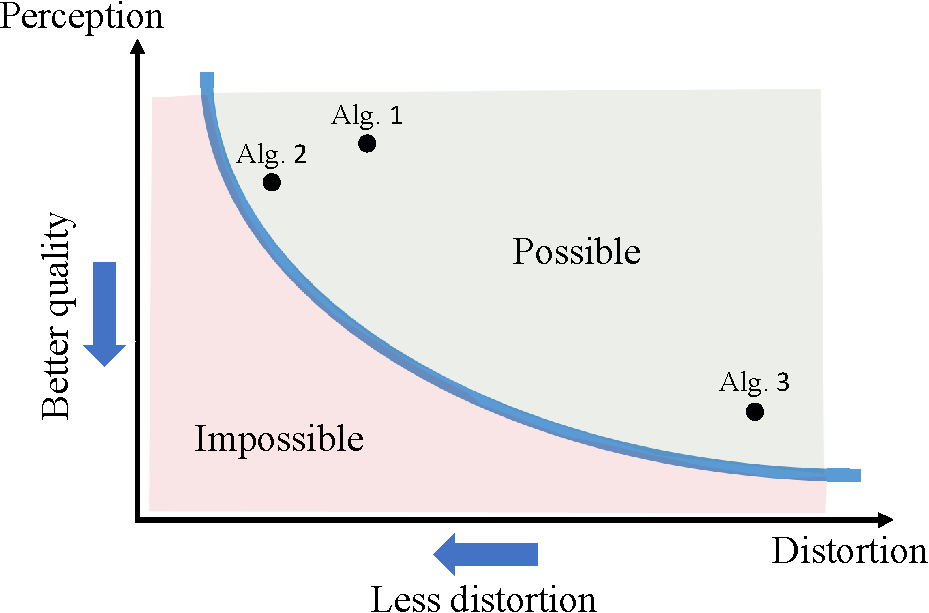
\includegraphics[width=0.87\linewidth]{figures/subObjPlane.pdf}
	\end{center}
	\caption{\textbf{The perception-distortion tradeoff.} Image restoration algorithms can be characterized by their average distortion and by the perceptual quality of the images they produce. We show that there exists a region in the perception-distortion plane which cannot be attained, regardless of the algorithmic scheme. When in proximity of this unattainable region, an algorithm can be potentially improved only in terms of its distortion \emph{or} in terms of its perceptual quality, one at the expense of the other.}
	\label{fig:subObjPlane}
\end{figure}

Based on these definitions of perception and distortion, we follow the logic of rate-distortion theory~\cite{cover2012elements}. That is, we seek to characterize the behavior of the best attainable perceptual quality (minimal deviation from natural image statistics) as a function of the maximal allowable average distortion, for any estimator. This perception-distortion function (wide curve in Fig.~\ref{fig:subObjPlane}) separates between the attainable and unattainable regions in the perception-distortion plane and thus describes the fundamental tradeoff between perception and distortion. Our analysis shows that algorithms cannot be simultaneously very accurate \emph{and} produce images that fool observers to believe they are real, no matter what measure is used to quantify accuracy. This tradeoff implies that optimizing distortion measures can be not only ineffective, but also potentially damaging in terms of visual quality. This has been empirically observed \eg in \cite{ledig2016photo,johnson2016perceptual,sajjadi2017enhancenet,yeh2017semantic,dahl2017pixel}, but was never established theoretically.

From the standpoint of algorithm design, we show that generative adversarial nets (GANs) provide a principled way to approach the perception-distortion bound. This gives theoretical support to the growing empirical evidence of the advantages of GANs in image restoration \cite{ledig2016photo,sajjadi2017enhancenet,pathak2016context,yeh2017semantic,rippel2017real,isola2016image,zhu2017unpaired}.


The perception-distortion tradeoff has major implications on low-level vision. In certain applications, reconstruction accuracy is of key importance (\eg medical imaging). In others, perceptual quality may be preferred. The impossibility of simultaneously achieving both goals calls for a new way for evaluating algorithms: By placing them on the perception-distortion plane. We use this new methodology to conduct an extensive comparison between recent super-resolution (SR) methods, revealing which SR methods lie closest to the perception-distortion bound. 